%!TEX root = ../book.tex
\section{Inverse Kinematics}\label{sec:kinematics:ik}

The forward kinematics of a system are computed by means of a transformation matrix from the base of a manipulator (or a corner of the room) to the end-effector of a manipulator (or a mobile robot).
As such, they are an exact description of the pose of the robot and they fully characterize its kinematic state.
Inverse Kinematics deal with the opposite problem, that is how to find a joint configuration that leads to a desired pose at the end effector.
To achieve this goal, we will need to solve the forward kinematics equations for joint angles as a function of the desired pose.
With reference to \cref{eq:kinematics:forward}, inverse kinematics aims to solve the following:
\begin{equation}\label{eq:kinematics:inverse}
q = f^{-1} (r)\ , \qquad f^{-1} : \mathbb{R}^m \rightarrow \mathbb{R}^n \ ,
\end{equation}
with a notation similar to \cref{eq:kinematics:forward}.
For a mobile robot, we can do this only for velocities in the local coordinate system, and need more sophisticated methods to calculate appropriate trajectories for the robot.

\subsection{Solvability}

\cref{eq:kinematics:inverse} is the inverted version of \cref{eq:kinematics:forward}, and as such is heavily non-linear.
Therefore, it makes sense to briefly think about whether we can solve it at all for specific parameters before trying.
Here, the workspace of a robot becomes important. The workspace is the sub-space that can be reached by the robot in any orientation.
Clearly, there will be no solutions for the inverse kinematic problem outside of the workspace of the robot.

A second question to ask is how many solutions we actually expect and what it means to have multiple solutions \textsl{geometrically}.
Multiple solutions to achieve a desired pose correspond to multiple ways in which a robot can reach a target.
For example a three-link arm that wants to reach a point that can be reached without fully extending all links (leading to a single solution), can do this by folding its links in a concave and a convex fashion.
How many solutions there are for a given mechanism and pose quickly becomes non-intuitive.
For example, a 6-DOF arm can reach certain points with up to $16$ different configurations!

\subsection{Inverse Kinematics of a Simple Manipulator Arm}\label{sec:kinematics:inverse:arm}

We will now look at the inverse kinematics of the $2-$link arm that we introduced in \cref{fig:fwk2dofarm}. We need to solve the equations determining the robot's forward kinematics by solving for $\alpha$ and $ \beta$.
This is tricky, however, as we have to deal with complicated trigonometric expressions.

To get an intuition, assume there to be only one link, $l_1$.  Solving (\ref{eq:cosxl1}) for $\alpha$ yields to two distinct solutions:

\begin{equation}
\alpha = \pm \cos^{-1}\frac{x_1}{l_1},
\end{equation}
as cosine is symmetric for positive and negative values.
Indeed, for any possible position on the $x-$axis ranging from $-l_1$ to $l_1$, there exist two solutions: the first one with the arm above the table, and the other one with the arm below it.
At the extremes of the workspace, both solutions are the same.

%\begin{verbatim}
%sol = Solve[Sin[a + b] + Sin[a] == y
%             && Cos[a + b] + Cos[a] == x,
%            {a, b}];
%min = sol /. {x -> 1, y -> 1}
%\end{verbatim}

Solving \ref{eq:fwk2dofarm} for $\alpha$ and $\beta$ adds two additional solutions that are cumbersome to reproduce here, involving terms of $x$ and $y$ to the sixth power, and is left as an exercise to the reader, for example using an online symbolic solver.


What will drastically simplify this problem, is to not only specify the desired position, but also the orientation $\theta$ of the end-effector. In this case, a desired pose can be specified in the following form
\begin{equation}
\left[
\begin{array}{cccc}
cos\theta & -sin\theta & 0 & x\\
sin\theta & cos\theta & 0 & y\\
0 & 0 & 1 & 0\\
0 & 0 & 0 & 1
\end{array}
\right].
\end{equation}
A solution can now be found by simply equating the individual entries of the transformation (\ref{eq:2armtrans}) with those of the desired pose. Specifically, we can observe:
\begin{eqnarray}
cos\theta &=& cos(\alpha+\beta)\\
\nonumber
x &=& \cos_{\alpha\beta}l_2+\cos\alpha l_1\\
\nonumber
y &=& \sin_{\alpha\beta}l_2+\sin\alpha l_1
\end{eqnarray}
These can be reduced to
\begin{eqnarray}
\theta &=& \alpha + \beta \nonumber \\
\cos\alpha &=& \frac{\cos_{\alpha\beta}l_2-x}{l_1}=\frac{\cos\theta l_2-x}{l_1} \\
\sin\alpha &=& \frac{\sin_{\alpha\beta}l_2-y}{l_1}=\frac{\sin\theta l_2-y}{l_1} \nonumber
\end{eqnarray}
Providing the orientation of the robot in addition to the desired position therefore allows solving for $\alpha$ and $\beta$ just as a function of $x$, $y$ and $\theta$.

The main issue with the geometric approach detailed above is that it does not scale easily with an increase of DoF at the joints, and and it quickly becomes unhandy with more dimensions.
For higher-DoF platforms, we can calculate a \textsl{numerical solution} using an approach that we will later see is very similar to path planning in mobile robotics.
To this end, we will first calculate a measure of error between the current solution and the desired one, and then optimize the joint configuration so as to minimize such error.
In our example, the measure of error is the Euclidian distance between the current end-effector pose as given by the forward kinematics equations in \cref{eq:fwk2dofarm} and the desired solution $[x,y]$ in configuration space, i.e.:
% To do this, you need to solve the forward kinematics for every point in configuration space and use the Euclidean distance to the desired target as height.
\begin{equation}\label{eq:kinematics:inverse:numerical}
f_{x,y}(\alpha,\beta)=\sqrt{\left(\sin_{\alpha\beta} + \sin_\alpha - y\right)^2 + \left(\cos_{\alpha\beta}+\cos_\alpha - x\right)^2}
\end{equation}
Here, the first two terms in the parentheses are given by the forward kinematics of the robot, whereas the third terms in the parentheses are the desired positions. For improved readability, we assume $l_1=l_2=1$.
\cref{eq:kinematics:inverse:numerical} is a 3D functional and can be plotted as a function of $\alpha$ and $\beta$, our joint-space variables.
% This is plotted for $\alpha=[-\pi/2,\pi/2]$ and $\beta=[-\pi,\pi]$ and $x=1$, $y=1$ in Figure~\ref{fig:inversekinematics}.
As shown in \cref{fig:inversekinematics}, this function has a minima, in this case zero, for values of $\alpha$ and $\beta$ that bring the manipulator to $(1,1)$. These values are $(\alpha \rightarrow 0, b \rightarrow -\frac{\pi}{2})$ and $(\alpha \rightarrow -\frac{\pi}{2}, b \rightarrow \frac{\pi}{2})$.

\begin{figure}
    \centering
        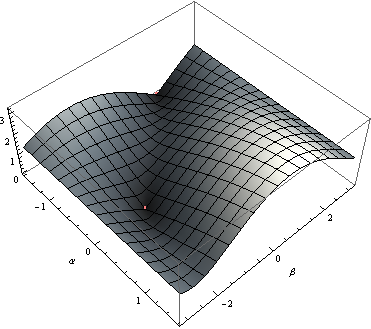
\includegraphics[width=0.8\textwidth]{figs/kinematics/inversekinematics}
    \caption{Distance to $(x=1,y=1)$ over the configuration space of a two-arm manipulator. Minima corresponds to exact inverse kinematic solutions.}
    \label{fig:inversekinematics}
\end{figure}

You can now think about inverse kinematics as a path finding problem from anywhere in the configuration space to the nearest minima. A formal approach to doing this will be discussed in \cref{sec:kinematics:inverse:feedbackcontrol}. How to find shortest paths in space, that is finding the shortest route for a robot to get from A to B will be a subject of chapter~\ref{chap:pathplanning}.


